\chapter{分布外检测}

\section{DML：为什么模型的置信度不等于模型对世界的认识程度？}

小孩不认识一张图片会说不认识——它不属于我训练过的知识。以往，许多 AI 模型即使看到完全没见过的东西，也可能非常自信地给出一个错误答案——因为它怎么着都能强行给一个答案，例如：

\begin{figure}[H]\centering
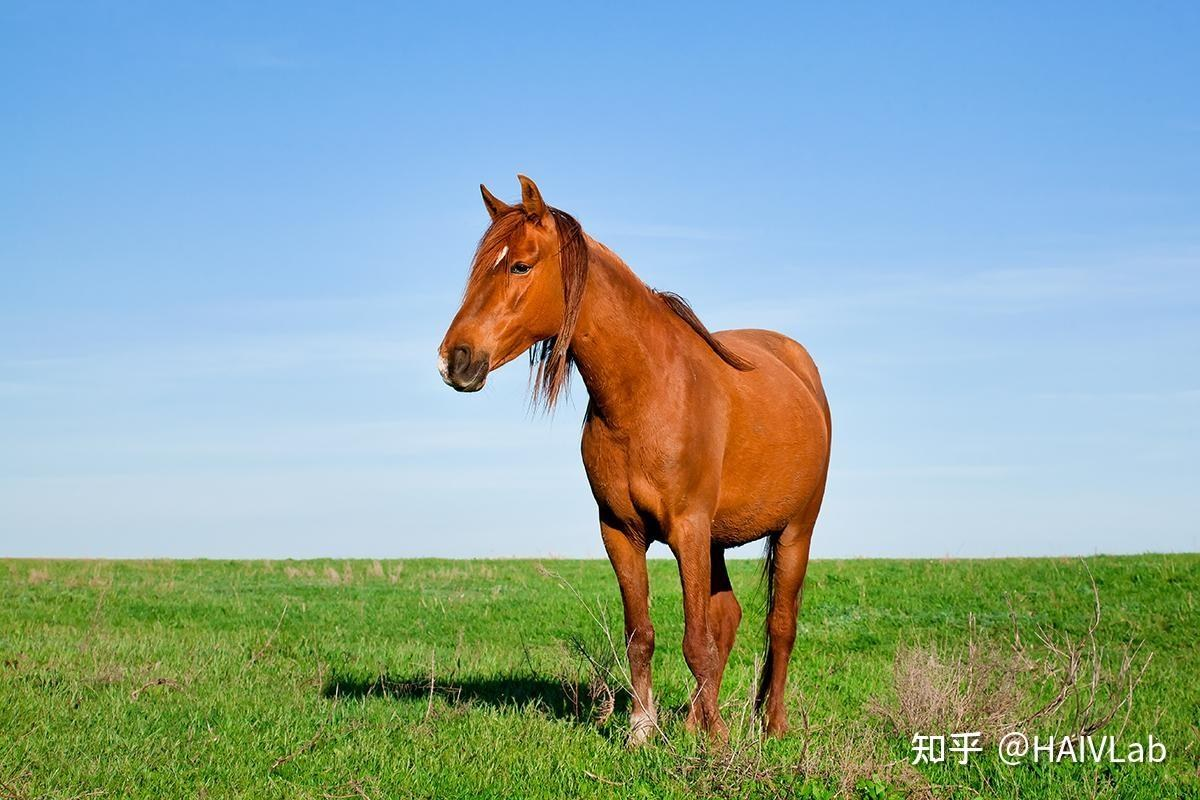
\includegraphics[width=0.82\linewidth,height=0.42\textheight,keepaspectratio]{figures/horse.jpg}
\caption*{训练内样本（ID）模型判断：马，置信度很高}
\end{figure}

\begin{figure}[H]\centering
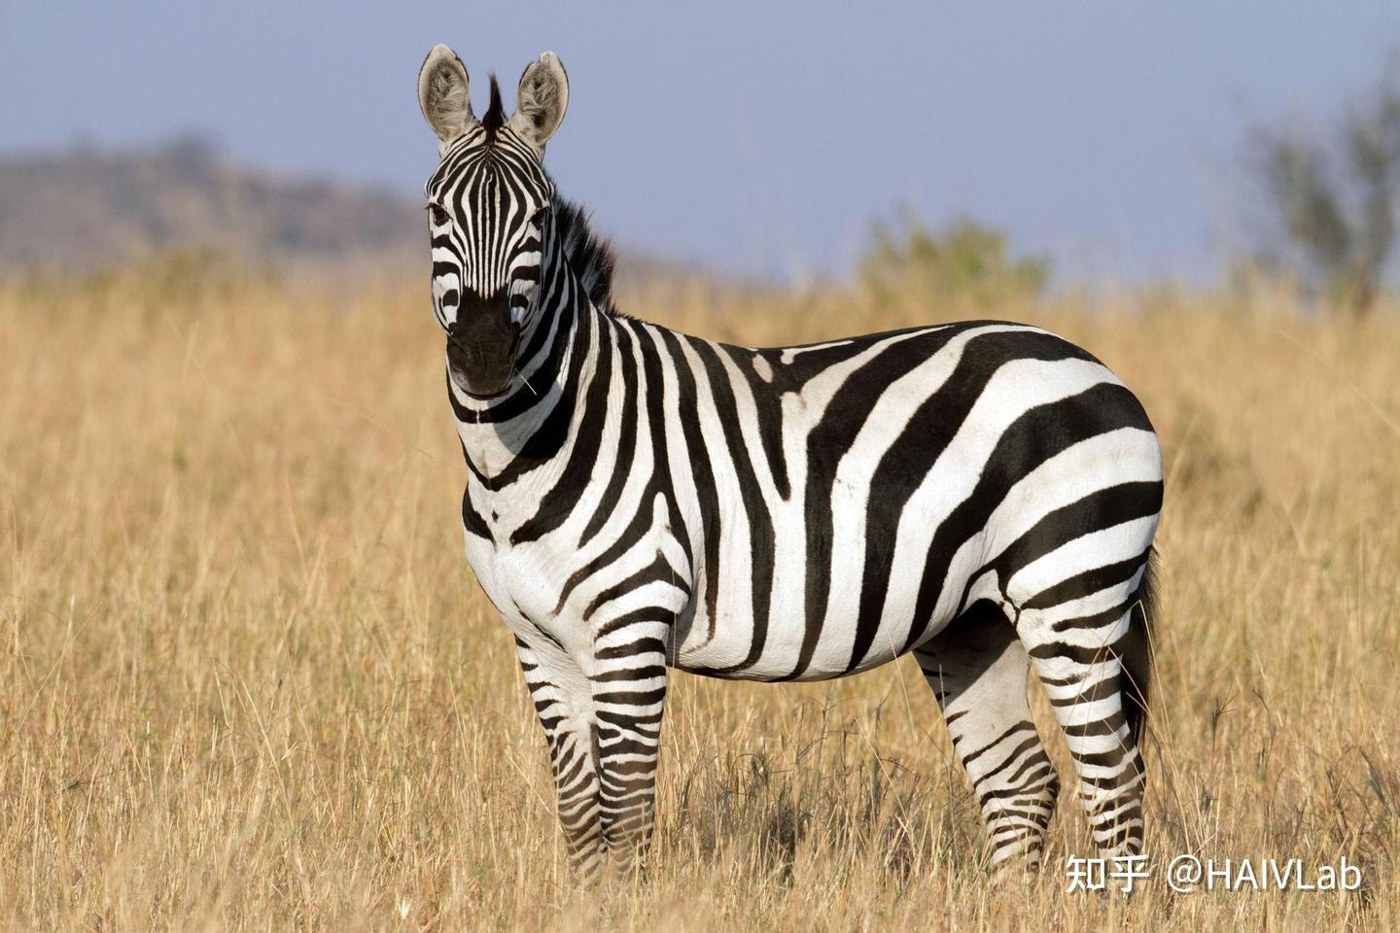
\includegraphics[width=0.82\linewidth,height=0.42\textheight,keepaspectratio]{figures/zebra.jpg}
\caption*{训练外样本（OOD）模型可能判断：马，置信度也很高}
\end{figure}

解决这种 AI 模型的问题，要用一类技术叫“分布外检测”——测试时样本是不是与训练样本同分布。以物体识别为例，因为分类器最后会输出一组数字（叫 Logits），一种简单且答题有效的分布外检测方法叫 MaxLogit—— 就是取最大的那个数字：

\[
S_{\mathrm{MaxLogit}}=\max_{k}\, z_k
\]

最大 Logit 越小，越可能是训练外样本。但 Logit 大小到底代表什么？

\[
z_k=\mathbf{w}_k^{\top}\mathbf{h}=\lVert\mathbf{w}_k\rVert\cdot\lVert\mathbf{h}\rVert\cdot\cos\theta_k
\]

MaxLogit 把方向和模长这两个因素混合在一起了。方向（Direction）衡量图片特征与某个类别的分类方向有多接近，最近称之为 MaxCosine。但我们通过实验观察到：方向和长度并不一定都能有效区分 ID 和 OOD。

MaxCosine：81.78\%

MaxNorm：56.93\%

MaxLogit：80.96\%

在 CIFAR-100，WRN-40-2 上，Norm 的作用并不大（AUROC，越高越好）：

\begin{enumerate}
  \item MaxCosine 本身比 MaxLogit 更有效。
  \item MaxNorm 单独使用效果很差。
  \item MaxNorm 与 MaxCosine 结合时，仍然可能提供补充信息。
\end{enumerate}

换句话说，MaxLogit 把有用的信息和不太有用的信息绑定在了一起。这就是Decoupling MaxLogit（DML）的初衷。不必再让它们以原来的方式相乘。

我们提出：

\[
\mathrm{DML}=\lambda\cdot\mathrm{MaxCosine}+\mathrm{MaxNorm}
\]

\begin{itemize}
  \item 主要依靠方向信息判断样本是否属于已知类别；
  \item 同时保留特征模长提供的辅助信息；
  \item 允许我们独立调节两者的重要程度。
\end{itemize}

这是一个 Post-hoc 方法：已有分类模型训练完成后，可以直接提取特征和分类器权重计算，不需要重新训练模型。简单有效（DML 比原始 MaxLogit 提高 1.38 个百分点）：DML：82.34\%

进一步，怎样让不太有效的 MaxNorm 更有效？可以引入额外训练，使用 Center Loss 可以让同一类别的样本特征尽量聚集在一起，这样特征模长也会更加稳定，MaxNorm 就更容易发挥作用。另一方面，使用 Focal Loss 可以更加关注那些难以分类的样本，而不是让模型只顾着把容易分类的样本训练得越来越好，这样可以减少困难样本对类别判别方向的干扰，让 MaxCosine 更有区分能力。再将普通 Linear Classifier 改成 Cosine Classifier，使分类更加关注特征方向，而不是单纯依靠增大特征模长来降低分类损失，就形成了最终版本 DML+。

DML+：93.16\%

\begin{itemize}
  \item Focal 模型负责提供更好的方向信息。
  \item Center 模型负责提供更好的模长信息。
  \item 最后把两个互补的信号结合起来。
\end{itemize}

总而言之，传统分类器把特征方向和特征模长混合在一个 Logit 里面，而这两个因素对OOD 检测的贡献并不相同。我们通过解耦这两种信息，并分别优化它们的表征能力，使一个非常简单的 Logit-based 方法获得了更好的 OOD 检测性能。

\paragraph{相关工作}

\begin{itemize}
  \item Zihan Zhang, Xiang Xiang*. Decoupling MaxLogit forOut-of-Distribution Detection. In CVPR, 2023.
\end{itemize}

\section{DPM：视觉语言模型如何认识未知？——从语义识别到分布认知}

在 DML：为什么模型的置信度不等于模型对世界的认识程度？中，识别模型还是卷积神经网络（CNN）——搭配传统分类器的话就只能在已知类别里面选一个。现在，普遍使用的识别模型是视觉语言模型（VLM）——在大规模图文数据上进行过预训练，类别甚广；且能同时理解图片和文字，图像识别的分类问题变成了图像与语义文本的匹配问题。

\begin{figure}[H]\centering
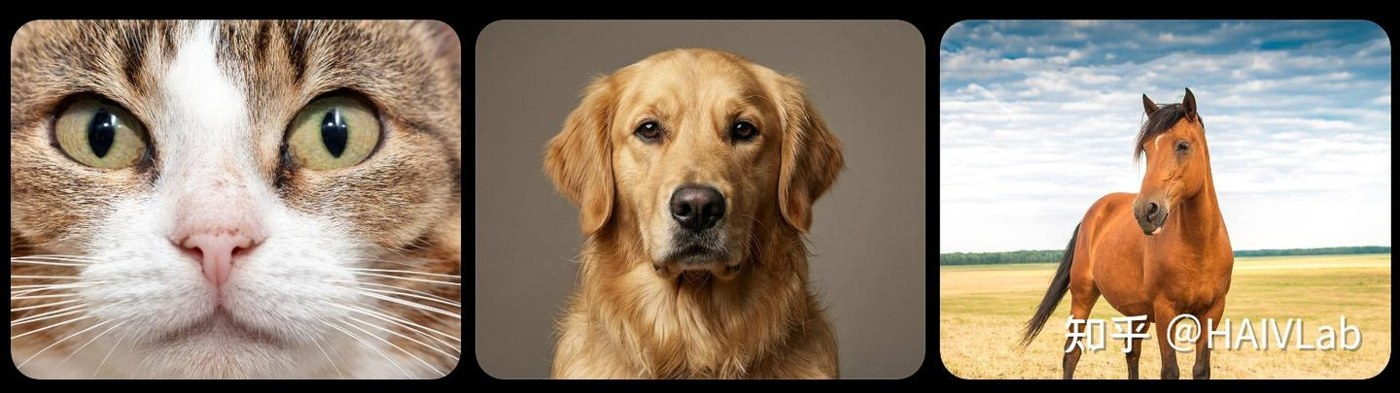
\includegraphics[width=0.82\linewidth,height=0.42\textheight,keepaspectratio]{figures/clip_cdh.jpg}
\caption*{对于“A photo of a cat. A photo of a dog. A photo of a horse.”，如果输入一张马的照片，CLIP 通常会认为它与 “A photo of a horse.” 的文本最相似。}
\end{figure}

但是，即便是 VLM，能给出一个语义上合理的答案，不等于对当前输入具有可靠的认知。并且，语义识别能力越强，越容易让我们忽略它实际上并不具备可靠的分布认知能力。例如，对于语义强大的 CLIP，分布外不应指模型从未见过的概念，而是判断测试样本是否服从当前下游任务定义的分布。例如，如果下游任务是 CIFAR-100 上的识别，CLIP 可能认识一只 CIFAR-100 之外的动物，但只要它不属于当前下游任务的 100 个类别，它仍然是分布外样本。

那么，对于 VLM，也可以做 DML 吗？以 CLIP 为例，原本就会对图像和文本特征分别进行 L2 Normalization（即使用 Cosine Similarity），因此若直接拿 CLIP 最终输出的图文相似度做 DML，实际上没有办法恢复原始的 Feature Norm 信息。

\begin{figure}[H]\centering
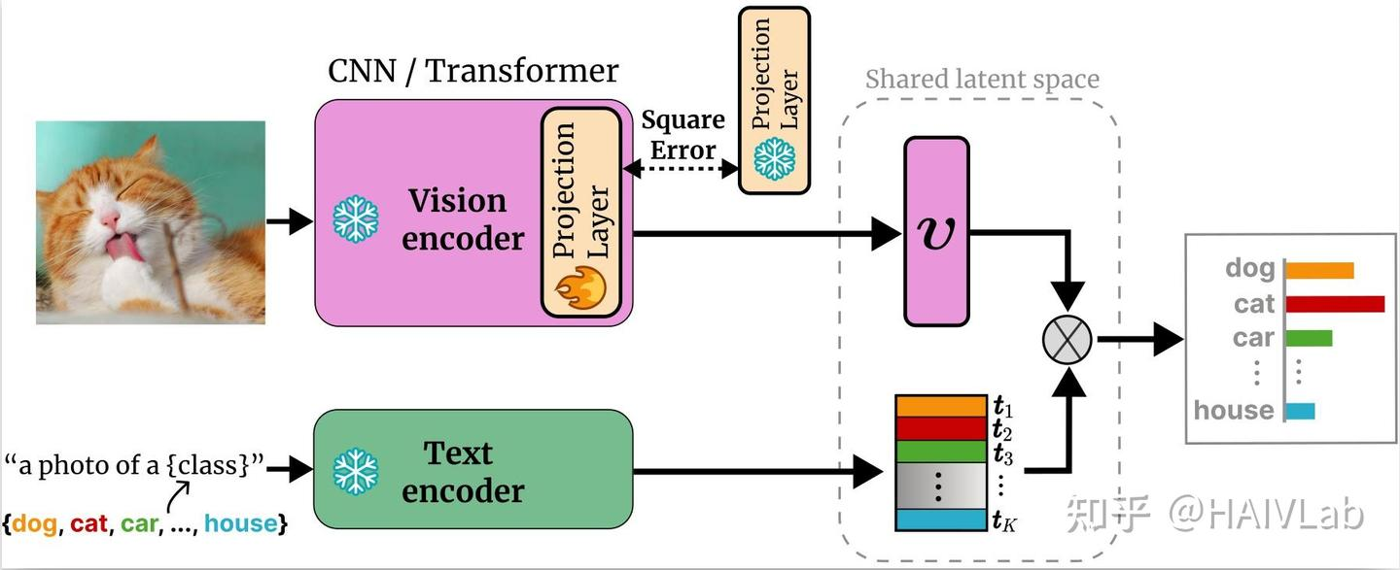
\includegraphics[width=0.82\linewidth,height=0.42\textheight,keepaspectratio]{figures/clip_arch.png}
\caption*{CLIP 用的是图文匹配分数}
\end{figure}

我们的初衷是分析不同信息的作用。对于 CLIP，要拆开的不是分类器的 Logit，而是文本信息与视觉信息。假设人要判断一张照片是不是一只猫，有两本参考资料：

\begin{figure}[H]\centering
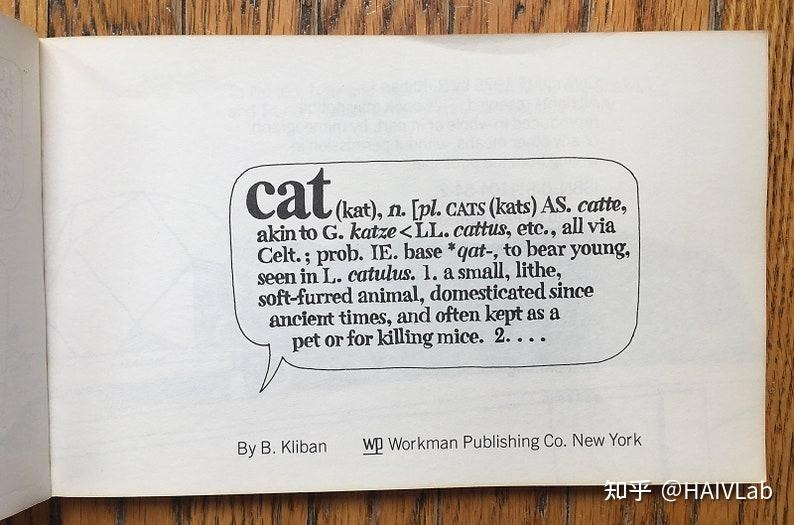
\includegraphics[width=0.82\linewidth,height=0.42\textheight,keepaspectratio]{figures/dict.jpg}
\caption*{文字描述：猫是一种有毛发、四条腿、胡须和尾巴的动物。}
\end{figure}

\begin{figure}[H]\centering
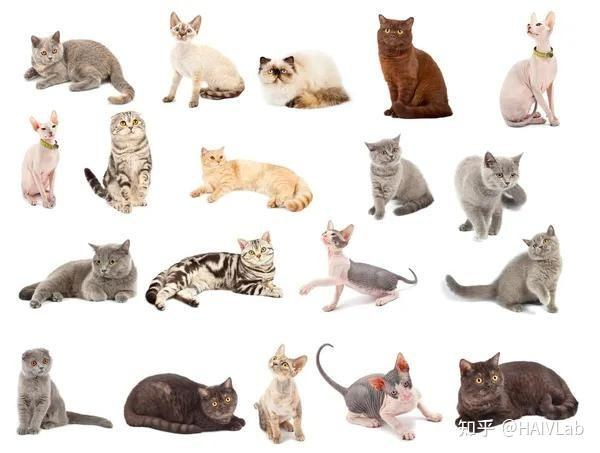
\includegraphics[width=0.82\linewidth,height=0.42\textheight,keepaspectratio]{figures/cats.jpg}
\caption*{过去见过的各种猫的图片：坐着的、躺着的；黑色的、白色的。}
\end{figure}

我们不仅可以利用视觉特征判断图片，还可以利用语言描述判断图片是否符合已知类别。

\subsubsection*{第一步：建立文本模式}

对于每个已知类别，我们准备一个文本描述。例如：

\begin{itemize}
  \item A photo of a cat.
  \item A photo of a dog.
  \item A photo of a horse.
\end{itemize}

利用 CLIP 的文本编码器，把它们变成特征向量，就是 Text Pattern 向量。

\subsubsection*{第二步：建立视觉模式}

我们把训练集里面的已知类别图片输入 CLIP。例如，对于每张猫的图片，计算它与所有已知类别文本的匹配分数。对这些结果取平均，就是猫类别对应的 Visual Pattern 向量，表达的是：一张真正属于猫类别的图片，通常会在所有类别上呈现怎样的匹配分布？对于狗、马也做同样的事情，就建立了一个视觉模式数据库。

\subsubsection*{第三步：测试时进行双重匹配}

现在来了一张测试图片。CLIP 先提取图片特征，然后分别进行两种比较：

Text Matching——与已知类别的文字特征比较，主要回答：这张图片在语义上像不像某个已知类别？

Visual Matching——与训练集形成的视觉模式比较，主要回答：这张图片的匹配行为，像不像这个类别在真实训练数据中的典型表现？

这种方式利用两种模态信息但依然简单，不需要修改 CLIP 参数——不需要训练，性能就已经超过了 MCM 和 ReAct。

总而言之，文字描述告诉我们一个类别在语义上是什么，但不一定能告诉我们这个类别在具体数据集里面长什么样。视觉模式正好补充了真实数据的分布信息，两者一结合就可以更好地识别那些语义上看起来合理、但视觉表现与已知数据存在差异的样本。凭借这个工作，我们从 CNN 时代的 DML 的改进 OOD Scoring，走向了 VLM 时代的 OODoriented Representation Learning。相关工作：

\begin{itemize}
  \item Zihan Zhang, Zhuo Xu, Xiang Xiang*: Vision-Language Dual-Pattern Matching forOut-ofDistribution Detection. In ECCV, 2024.
  \item Xiang Xiang*, Zhuo Xu, Zihan Zhang, Zhigang Zeng, Xilin Chen: Enhanced Dual-Pattern
\end{itemize}

Matching with Vision-Language Representation forOut-of-Distribution Detection. IEEE Trans. PAMI, 2025.

\section{ASL：既然方向很重要，能不能在训练阶段塑造更好的角度空间？}

\begin{figure}[H]\centering
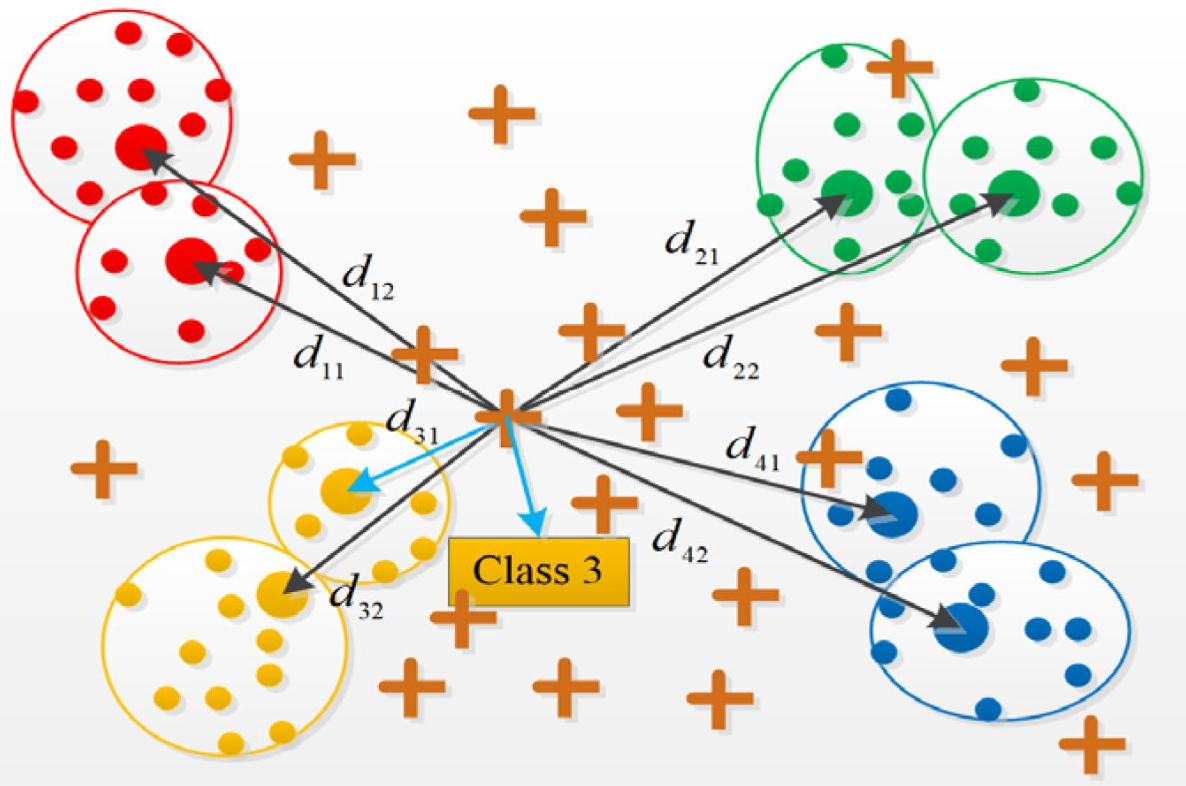
\includegraphics[width=0.82\linewidth,height=0.42\textheight,keepaspectratio]{figures/asl_dist.png}
\end{figure}

在 DML：为什么模型的置信度不等于模型对世界的认识程度？中，我们揭示了在分类器 Logit 输出中，特征模长和方向包含不同的分布外检测（OOD）信息。另一种 OOD的思路不直接看分类器输出，而是观察模型内部提取的特征。例如，训练数据中有猫、狗、汽车三个类别。我们可以计算每个类别在特征空间中的分布中心。对于一张新图片，如果特征落在某个已知类别的分布附近，判断为 ID；如果远离所有已知类别的分布，判断为 OOD。

涉及到距离，传统的 Mahalanobis Distance 同时考虑方向和模长。于是，一个 OOD 样本即使方向上明显偏离了已知类别，只要它的特征模长足够小，仍然可能在马氏距离计算中显得非常接近 ID 类别中心。这意味着，OOD 样本可以钻特征模长的空子。这远不是我们第一次关注角度与模长，除了在 DML 里，早在 2017 年 NormFace 工作中，我们就通过 L2 normalization 控制特征模长，让判别更多依赖角度关系。有鉴于此，对于OOD 其实以前已经有人注意到了特征模长的问题。例如 MD++，它尝试在计算Mahalanobis Distance 之前，对特征进行归一化。

但这样还不够，因为归一化只能改变测试时的距离计算方式，并不能改变模型训练时学到的特征空间结构。什么叫特征空间？在特征空间里，近的应该是语义接近。Mahalanobis Distance 是空间距离度量方式，但对于 OOD，空间距离并不总是等于语义上的接近程度。本质问题其实是，我们需要在训练时学到一个更好的特征空间——特别是如果特征模长归一化了，就是要学到一个更好的角度空间。

ASL 的思想非常简单。以前的标准分类训练是：

\[
\begin{gathered}x\rightarrow\mathrm{Encoder}\rightarrow\mathrm{Feature}\rightarrow\mathrm{Linear\ Classifier} \\ x\rightarrow\mathrm{Encoder}\rightarrow\mathrm{Feature}\rightarrow\mathrm{L2\ Normalization}\rightarrow\mathrm{Linear\ Classifier}\quad(\text{ASL})\end{gathered}
\]

类似 MD++，ASL 在 Feature 和 Classifier 之间增加一个 L2 Normalization，分类器就不能再依靠不断增大 Feature Norm 来降低分类损失，而必须更多地依靠特征方向来区分类别。然后，使用普通的 Cross-Entropy，就可以在角度空间中实现一种基于类别原型的对比学习。例如，训练一张猫的图片时，猫的特征方向要靠近猫的权重向量同时要远离狗和汽车的权重向量，实际上就完成了：

\begin{enumerate}
  \item 类内角度聚集；
  \item 类间角度分离；
  \item 在单位球面上形成更清晰的类别结构。
\end{enumerate}

\begin{figure}[H]\centering
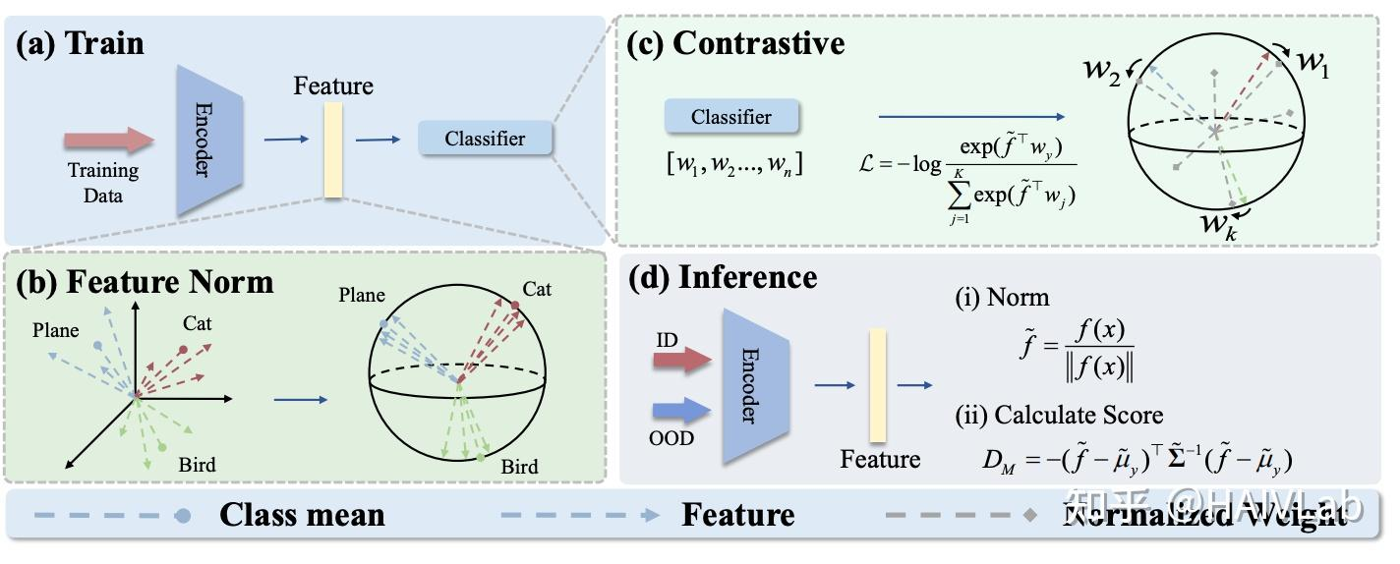
\includegraphics[width=0.82\linewidth,height=0.42\textheight,keepaspectratio]{figures/asl_fw.png}
\caption*{特征归一化后再用 CE 训练，本身就有对比学习的效果}
\end{figure}

不需要额外构造负样本，也不需要复杂的 Contrastive Loss，就得取得很好的 OOD 性能。ImageNet-200，ResNet-18，从头训练

Cross-Entropy：82.8\%

ReweightOOD：83.7\%

T2FNorm：83\%

ASL：85.1\%

（均为 Near-OOD 平均 AUROC，越高越好）

ImageNet-1K，ViT-B/16

\begin{table}[H]\centering
\caption*{ImageNet-1K，ViT-B/16}
\begin{tabular}{lll}\toprule
\textbf{方法} & \textbf{Near-OOD AUROC} & \textbf{Far-OOD AUROC} \\ \midrule
Cross-Entropy & 78.5\% & 91.9\% \\
ASL & 81.9\% & 94.0\% \\
\bottomrule\end{tabular}
\end{table}

ASL 不只是提高 OOD Detection，还保持了相近的分类准确率。例如在 CIFAR-10 上：

\begin{itemize}
  \item 标准 CE：95.2\% 分类准确率。
  \item ASL：94.8\% 分类准确率。
\end{itemize}

说明它没有通过简单牺牲分类能力换取 OOD 检测效果。总而言之，ASL 直接改变训练方式，让模型从一开始就学习更适合 OOD 检测的特征空间——用非常简单的操作实现角度空间的对比学习（没有额外的负样本生成，没有复杂的样本挖掘，也没有额外的对比损失）。DML 并不是简单地认为 Feature Norm 没有价值而是尝试把方向和模长分别利用；而 ASL 针对 Mahalanobis Distance 这一类距离检测器中的模长干扰问题，选择在训练阶段弱化模长对分类学习的影响。两条线索最终汇合在一个问题上：模型内部的特征表示，究竟能否真实反映输入与已知数据分布之间的关系？两者并不矛盾，而是针对不同检测机制提出了不同解决方案。ASL 说，与其在一个不理想的特征空间里不断修补检测算法，不如直接改变模型学习特征空间的方式。

\paragraph{相关工作}

\begin{itemize}
  \item Hanlin Li, Jing Ma, Zehang Wei, Jiamin Yan, Xiang Xiang*. Why Feature Magnitude Deceives OOD Detectors: An Angular Separation Perspective. In ECCV, 2026.
  \item Feng Wang*, Xiang Xiang*, Jian Cheng, Alan Yuille: NormFace: L2 Hypersphere Embedding for Face Verification. In ACM Multimedia, 2017.
\end{itemize}

\section{OSPCoOp: 从识别未知类别，到识别模型判断中的错误依据}

在《DPM：视觉语言模型如何认识未知？——从语义识别到分布认知》中，我们思考文本语义是否足以代表下游任务的视觉分布，于是提出 Text Pattern + Visual Pattern。作为信息分析流派，我们总是在拆开特征的组成成分——Text vs Visual (DPM)，方向 vs 模长（DML, ASL, NormFace），等等。现在，以 CLIP 为例，我们进一步思考 CLIP 真的识别了图像中的语义吗？

在 2024 年，我们发现：CLIP 有时可能认的是背景，而不是物体。看来我们又要拆开物体特征 vs 背景特征了！假设我们用 ImageNet-1K 训练一个下游识别任务，其中有一个类别叫 Grey Whale（灰鲸）。正常情况下，图片里有一头灰鲸，CLIP 会给 Grey Whale 很高的匹配分数。

\begin{figure}[H]\centering
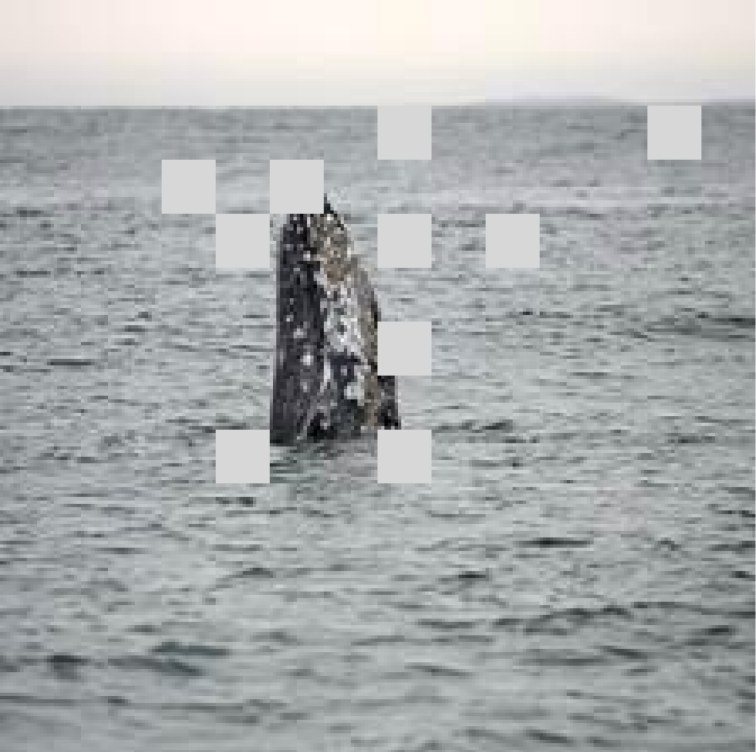
\includegraphics[width=0.82\linewidth,height=0.42\textheight,keepaspectratio]{figures/whale.jpg}
\end{figure}

\begin{figure}[H]\centering
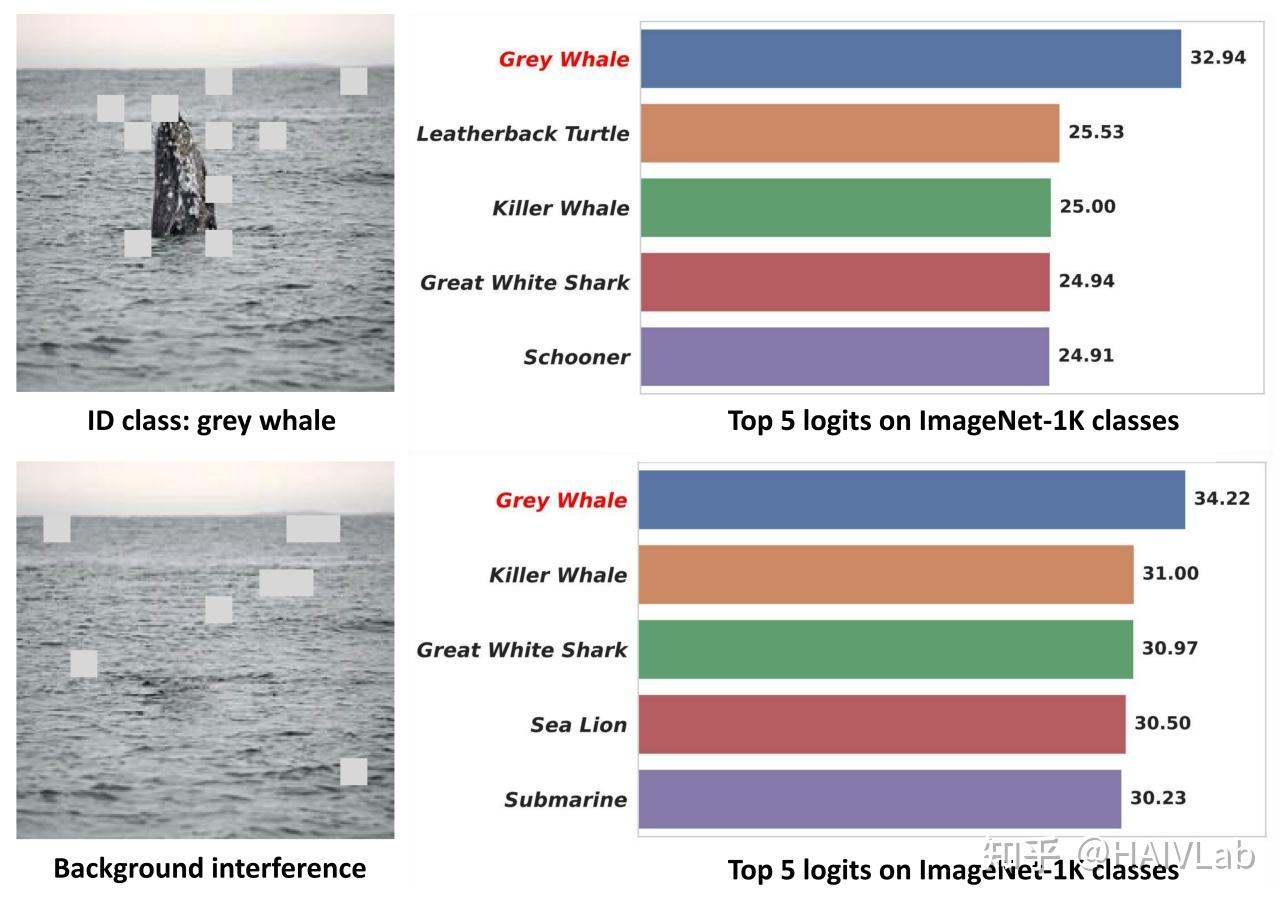
\includegraphics[width=0.82\linewidth,height=0.42\textheight,keepaspectratio]{figures/whale_bar.png}
\caption*{把鲸鱼从图片中去掉，CLIP 给 Grey Whale 的分数比原图还高}
\end{figure}

如果把鲸鱼从图片中去掉，只留下海水等背景区域，CLIP 仍然可能给 Grey Whale 很高的分数，甚至比原图还高。这不难解释——在训练数据中，灰鲸经常出现在海洋环境里。模型可能学到了一个捷径：看到海洋背景，就倾向于判断为灰鲸。于是，模型并不一定真正依赖鲸鱼本身的视觉特征，而是利用了背景与类别之间的统计关联——类似走捷径 Shortcut Learning。这和传统意义上模型认错一只动物还不完全一样，这里更重要的问题是：模型可能通过一个不可靠的背景线索，判断一张本来应该被识别为OOD 的图片属于 ID。例如，模型在海洋背景上学会了灰鲸这个类别，那么一张只有海水、船只或其他海洋场景的图片，也可能被错误地接纳为分部内（In-Distribution, ID）。这就暴露出一个问题：VLM 的语义能力很强，但它并不意味着模型真正理解了图像中哪些区域对当前任务有用。

为了 Overcoming Shortcut Learning (OSP)，我们提出 OSPCoOp（OSP via Convex Optimization）。核心不是简单地增加 OOD 类别，而是从图像中分离出两类区域：

\begin{itemize}
  \item ID-relevant regions：与当前 ID 类别识别有关的区域，例如鲸鱼主体。
  \item ID-irrelevant regions：对当前 ID 类别识别不重要的区域，例如背景海水。
\end{itemize}

然后第一步：利用背景制造伪 OOD 样本。先把训练图片中的主体区域和背景区域拆开。再把背景区域拿出来，经过增强，构造出大量背景 OOD 样本。这样，模型就能看到：即使背景来自一张原本属于 ID 的图片，单独出现时也不应该被判断为 ID。这一步没有依赖人工收集大量真正未知类别，而是从现有 ID 数据中挖掘出一种容易被模型误判的OOD 样本。

第二步：用 mask 约束模型关注哪里。仅仅告诉模型背景是 OOD 还不够——模型可能仍然依赖背景线索。利用前面得到的区域 mask，对模型的注意力进行约束，让模型减少对 ID-irrelevant 区域的关注，更多利用与类别相关的视觉区域。

使用 CLIP 的 ViT-B/32 和 ResNet-50 等架构进行验证。几个关键结果很有说服力：

\begin{table}[H]\centering
\caption*{OSPCoOp 主要结果}
\begin{tabular}{ll}\toprule
\textbf{实验} & \textbf{OSPCoOp 结果} \\ \midrule
ImageNet-1K ID，16-shot，传统 OOD 平均 AUROC & 93.64\% \\
ImageNet-Bg，AUROC & 91.37\% \\
传统 OOD，1-shot 平均 AUROC & 93.81\% \\
\bottomrule\end{tabular}
\end{table}

在 ImageNet-Bg 上，和我们之前的 DPM 比较：

\begin{table}[H]\centering
\caption*{ImageNet-Bg 上与 DPM 的比较}
\begin{tabular}{ll}\toprule
\textbf{方法} & \textbf{AUROC $\uparrow$} \\ \midrule
DPM-F & 89.53 \\
OSPCoOp & 91.37 \\
\bottomrule\end{tabular}
\end{table}

在传统四类 OOD 数据集的 16-shot 实验中，OSPCoOp 的平均 AUROC 为 93.64\%，也超过LoCoOp 的 91.20\% 和 SCT 的 91.86\%。

总而言之，OSPCoOp 改变了 OOD 评测的视角：不再只问模型能不能识别未知物体，还要问模型能不能拒绝那些仅仅具有分部内背景特征的图片。模型做出正确判断，究竟是因为理解了真正有意义的信息，还是因为找到了一个与答案相关、但并不可靠的线索？这个问题远远超出了背景识别，后来我们看到了很多类似的探索与发现，例如在医学影像分析中，模型是否利用了医院设备、扫描仪或图像附加标记（甚至不用看影像），而不是真正的病灶？这也让 OOD 检测的含义更深了一层。以前我们主要思考模型是否见过这个类别？现在还要思考模型判断这个类别的依据是否可靠？必要的情况下我们需要拆开这些依据。当然，OSPCoOp 也有自己的边界：它重点处理的是前景与背景之间的捷径问题，并不解决所有形式的 shortcut learning；而且它依赖外部区域分割和背景处理的质量。

\paragraph{相关工作}

\begin{itemize}
  \item Zhuo Xu, Xiang Xiang*, Yifan Liang: Overcoming Shortcut Problem in VLMs for RobustOutof-Distribution Detection. In CVPR, 2025. (Spotlight)
\end{itemize}
